\subsection{Confirmatory run: 13 scenes and the extensions}\label{sec:v2}
The first ETH3D run exposed two weaknesses: bounds that under-cover under degradation, most of all on hard cameras, and too few test scenes for significance. We designed E1 and E2 (\cref{sec:ext}) on the calibration scenes of that run, with injected failures and leave-one-scene-out validation, and then evaluated them on its test scenes, which had been seen in aggregate before. To test them without that bias, we computed a second, independent set of VGGT outputs and fixed six hypotheses, the primary variant and all settings before those outputs existed (the pre-registration file is reproduced in \supp{7} and released with the code). The development of E1 and E2 and their results on the first run are in \supp{5}, and their behaviour on synthetic scenes in \supp{6}.

\paragraph*{Protocol (E4)} All 13 ETH3D scenes are test scenes in turn: for each, CARA is calibrated on 140 clean sub-scenes of the other 12 scenes (leave-one-scene-out) and tested on 8 new random sub-scenes of 12 cameras (seed 3, none shared with the first run) under the same 7 conditions, 728 test graphs in total (21 of them keep 7 or 11 cameras after restriction to the largest component). Seven of the 13 places are the first run's test scenes, with different images selected. Each file also stores VGGT's relative translation, the relative rotation of the previous camera-head iteration, and per-image confidence statistics. Everything else follows \cref{sec:eth3d}; the unit of inference is the test scene (13 scenes, smallest two-sided $p=2^{-12}$). The clean edges have a median inlier error of $0.74^\circ$, 21.1\% exceed $5^\circ$ and 11.7\% exceed $30^\circ$; under low light at $0.15$ the latter reaches 19.4\%.

\paragraph*{E3: learned edge uncertainty} From the stored signals we form five edge features (median confidence over both images, the worst and the best image's mean log confidence, the worst image's 10\% confidence quantile, and the log angle between the last two camera-head iterations) and fit $\log\hat\sigma$ as a linear function of them to the log error of inlier edges on $\mathcal{D}_{\mathrm{fit}}$ only. For numerical safety the prediction is clipped to $[10^{-4},\pi]$\,rad. This guard was added after the run-2 outputs had been computed and the first evaluation attempt failed on a fold that produced a zero uncertainty; it changes no other setting, but it is a deviation from the pre-registration. Separating outlier edges ($>5^\circ$), the learned $\hat\sigma$ reaches an AUROC of $0.873$ against $0.701$ for the pre-registered median (13 of 13 scenes). The worst-image mean log confidence alone reaches $0.853$ and, unexpectedly, the small change between camera-head iterations (median $0.028^\circ$, quantized by the half-precision arithmetic of the T4 GPU) reaches $0.824$; the 10\% quantile sits on VGGT's confidence floor and carries no information ($0.505$).

\begin{table*}[!htbp]\centering\footnotesize
\caption{Confirmatory ETH3D run (13 scenes, leave-one-scene-out calibration, 8 new sub-scenes of 12 cameras per scene and condition, 5 calibration seeds): AUC@5$^\circ$, mean over test scenes with 95\% bootstrap interval. -L: learned edge uncertainty (E3). Best per row in bold.}\label{tab:v2acc}
\setlength{\tabcolsep}{2.5pt}\resizebox{\textwidth}{!}{\begin{tabular}{lcccccccc}\toprule
Condition & CG & GLOMAP-RA & Shonan-H & CG-$\hat\rho$ & ConfW & CARA & ConfW-L & CARA-L \\\midrule
clean & 0.645\,{\scriptsize[0.554,0.733]} & 0.649\,{\scriptsize[0.558,0.738]} & 0.610\,{\scriptsize[0.515,0.708]} & 0.638\,{\scriptsize[0.549,0.727]} & 0.685\,{\scriptsize[0.604,0.762]} & 0.665\,{\scriptsize[0.594,0.740]} & \textbf{0.722\,{\scriptsize[0.642,0.793]}} & 0.707\,{\scriptsize[0.630,0.781]} \\
fog 0.7 & 0.635\,{\scriptsize[0.548,0.718]} & 0.634\,{\scriptsize[0.541,0.720]} & 0.583\,{\scriptsize[0.483,0.684]} & 0.626\,{\scriptsize[0.538,0.711]} & 0.681\,{\scriptsize[0.610,0.754]} & 0.666\,{\scriptsize[0.589,0.737]} & \textbf{0.695\,{\scriptsize[0.626,0.761]}} & 0.677\,{\scriptsize[0.590,0.755]} \\
fog 0.5 & 0.610\,{\scriptsize[0.521,0.703]} & 0.596\,{\scriptsize[0.507,0.689]} & 0.550\,{\scriptsize[0.452,0.648]} & 0.606\,{\scriptsize[0.517,0.696]} & 0.649\,{\scriptsize[0.571,0.725]} & 0.639\,{\scriptsize[0.562,0.715]} & \textbf{0.682\,{\scriptsize[0.584,0.764]}} & 0.662\,{\scriptsize[0.577,0.743]} \\
fog 0.3 & 0.593\,{\scriptsize[0.496,0.690]} & 0.574\,{\scriptsize[0.471,0.673]} & 0.545\,{\scriptsize[0.445,0.644]} & 0.591\,{\scriptsize[0.482,0.693]} & 0.620\,{\scriptsize[0.526,0.710]} & 0.624\,{\scriptsize[0.541,0.707]} & \textbf{0.653\,{\scriptsize[0.556,0.741]}} & 0.624\,{\scriptsize[0.540,0.708]} \\
low 0.3 & 0.509\,{\scriptsize[0.379,0.634]} & 0.513\,{\scriptsize[0.384,0.640]} & 0.471\,{\scriptsize[0.338,0.596]} & 0.506\,{\scriptsize[0.383,0.626]} & 0.540\,{\scriptsize[0.413,0.657]} & 0.541\,{\scriptsize[0.424,0.657]} & \textbf{0.571\,{\scriptsize[0.447,0.691]}} & 0.566\,{\scriptsize[0.453,0.679]} \\
low 0.15 & 0.494\,{\scriptsize[0.356,0.627]} & 0.485\,{\scriptsize[0.358,0.604]} & 0.452\,{\scriptsize[0.323,0.571]} & 0.488\,{\scriptsize[0.355,0.611]} & 0.507\,{\scriptsize[0.370,0.635]} & 0.520\,{\scriptsize[0.393,0.635]} & 0.540\,{\scriptsize[0.407,0.662]} & \textbf{0.552\,{\scriptsize[0.432,0.664]}} \\
rain & 0.547\,{\scriptsize[0.452,0.630]} & 0.544\,{\scriptsize[0.454,0.629]} & 0.528\,{\scriptsize[0.434,0.617]} & 0.546\,{\scriptsize[0.451,0.630]} & 0.545\,{\scriptsize[0.447,0.633]} & 0.559\,{\scriptsize[0.473,0.637]} & 0.564\,{\scriptsize[0.465,0.650]} & \textbf{0.565\,{\scriptsize[0.474,0.651]}} \\
\bottomrule\end{tabular}}\end{table*}


\paragraph*{Accuracy with 13 scenes} \Cref{tab:v2acc} reports AUC@5$^\circ$. With the pre-registered $\hat\sigma$, CARA's mean is above CG in all seven conditions (by $0.012$ to $0.032$) and above GLOMAP-RA and Shonan-H in all seven. Over the 13 scenes, pooled across conditions, CARA beats CG on 9 scenes ($+0.026$, $p=0.051$), GLOMAP-RA on 10 ($p=0.028$), Shonan-H on 10 ($p=0.002$) and CG-$\hat\rho$ on 9 ($p=0.037$). These comparisons were not among the pre-registered hypotheses and are not corrected for multiplicity. ConfW remains as accurate as CARA ($-0.002$, $p=0.84$). With the learned $\hat\sigma$ (E3), CARA gains $0.020$ (11 of 13 scenes, $p=0.018$; not in fog $0.3$) and ConfW gains $0.029$; the most accurate method in five of seven conditions is ConfW with the learned uncertainty, and CARA with it is not significantly different ($-0.010$, $p=0.33$). Better uncertainty helps both uncertainty-aware methods we tested; CARA's gates do not add accuracy on top of good weights.

\begin{table}[!htbp]\centering\footnotesize
\caption{Per-camera bounds (target 90\%) in the confirmatory run: coverage of registered cameras, coverage on the quarter with the largest $u_i$ (hard), median width of unflagged bounds, fraction of cameras flagged (bound $>30^\circ$), and fraction of catastrophic cameras ($>30^\circ$) that are flagged. Means over 13 test scenes and 5 seeds.}\label{tab:v2bounds}
\setlength{\tabcolsep}{2.2pt}\begin{adjustbox}{max width=\textwidth}\begin{tabular}{llccccc}\toprule
 & Variant & cov. & hard & width$^\circ$ & flagged & cat.\ flagged \\\midrule
\multirow{6}{*}{clean} & base & 0.898 & 0.837 & 15.3 & 0.265 & 0.430 \\
 & E1 & 0.911 & 0.856 & 19.6 & 0.393 & 0.535 \\
 & E2 & 0.923 & 0.922 & 6.8 & 0.326 & 0.816 \\
 & E2u & 0.925 & 0.924 & 8.9 & 0.517 & 0.764 \\
 & E1+E2a & 0.903 & 0.869 & 9.1 & 0.146 & 0.559 \\
 & E1+E2 & 0.883 & 0.891 & 4.6 & 0.229 & 0.706 \\
\midrule
\multirow{6}{*}{degraded} & base & 0.879 & 0.818 & 15.6 & 0.356 & 0.450 \\
 & E1 & 0.894 & 0.842 & 19.8 & 0.489 & 0.606 \\
 & E2 & 0.909 & 0.928 & 8.1 & 0.416 & 0.781 \\
 & E2u & 0.925 & 0.925 & 8.4 & 0.609 & 0.727 \\
 & E1+E2a & 0.882 & 0.853 & 10.6 & 0.212 & 0.546 \\
 & E1+E2 & 0.867 & 0.893 & 5.1 & 0.310 & 0.671 \\
\bottomrule\end{tabular}\end{adjustbox}\end{table}


\paragraph*{Per-camera bounds} \Cref{tab:v2bounds} pools the six degraded conditions, and \cref{fig:v2}(a) shows each condition. The unmodified bounds cover 87.9\% of registered cameras and 81.8\% of the hardest quarter; with leave-one-scene-out calibration over 12 varied scenes they are wide (median $15.6^\circ$ when not flagged) and flag 36\% of cameras. E2 raises coverage on the hardest quarter to 92.8\% ($+11.0$ points, 11 of 13 scenes) and overall coverage to 90.9\% ($+3.1$, 7 of 13 scenes), halves the unflagged width to $8.1^\circ$, and flags 78\% of the cameras whose error exceeds $30^\circ$, against 45\% without it. The cost is a higher flag rate (42\% against 36\%): only about one flagged camera in five is actually wrong by more than $30^\circ$, so on these small graphs a 90\% guarantee is bought by declaring many correct cameras unreliable. E1 alone adds 1.5 points of coverage (12 of 13 scenes) at the price of wider bounds. Combining E1 with E2 gives narrower bounds and fewer flags (31\%) but covers less than E2 alone, and less than the unmodified bounds overall (86.7\%). E1+E2a denotes E1 with the learned normalizer but without groups. The secondary variant E2u, which groups cameras by $u_i$ without the learned normalizer, covers more than E2 (92.5\% overall and on hard cameras; hard coverage above the unmodified bounds on all 13 scenes) but flags 61\% of cameras. As in the first run, the learned normalizer does not rank catastrophic cameras better than $u_i$ (AUROC $+0.002$); its benefit is a better split into groups.

\begin{figure}[!htbp]\centering
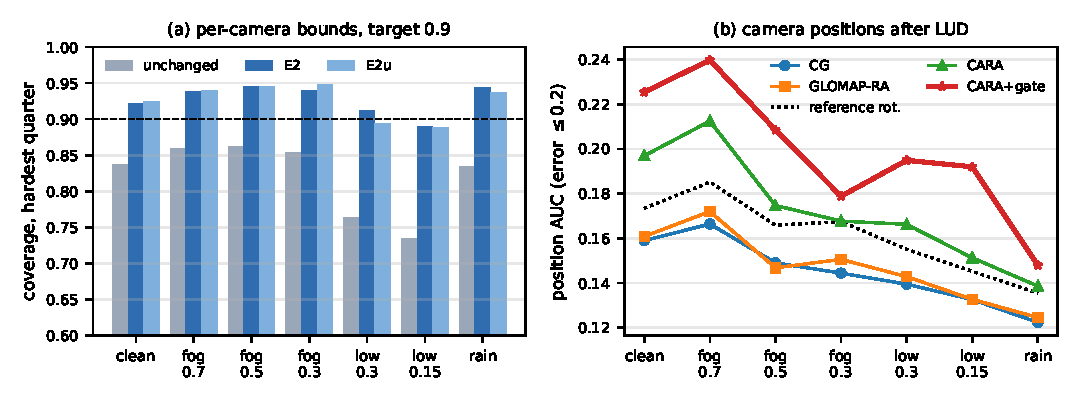
\includegraphics[width=\linewidth]{figs/v2.pdf}
\caption{Confirmatory ETH3D run (13 scenes). (a) Coverage of the per-camera bounds on the quarter of cameras with the largest $u_i$, for the unchanged bounds and the difficulty-conditional variants E2 and E2u; dashed line: target. (b) Position AUC after translation averaging by least unsquared deviations (LUD) with each method's rotations; CARA+gate uses only CARA's accepted edges, and the dotted line uses the reference rotations with all edges.}\label{fig:v2}
\end{figure}

\begin{table}[!htbp]\centering\footnotesize
\caption{Downstream camera positions (E5): LUD translation averaging of VGGT's relative translations, rotated by each method's global rotations. AUC of the scale-free position error up to $0.2$ (higher is better) and its median (lower is better); +gate uses only CARA's accepted edges. GT rot.\ uses the reference rotations and all edges.}\label{tab:v2trans}
\setlength{\tabcolsep}{2pt}\resizebox{\columnwidth}{!}{\begin{tabular}{lcccccc}\toprule
 & GT rot. & CG & GLOMAP-RA & CARA & CARA+gate & CARA-L+gate \\\midrule
clean & 0.173/0.32 & 0.159/0.37 & 0.161/0.38 & 0.197/0.33 & 0.225/0.33 & 0.233/0.32 \\
fog 0.7 & 0.185/0.34 & 0.166/0.39 & 0.172/0.39 & 0.212/0.36 & 0.240/0.34 & 0.227/0.35 \\
fog 0.5 & 0.166/0.35 & 0.149/0.41 & 0.147/0.42 & 0.175/0.39 & 0.208/0.36 & 0.202/0.37 \\
fog 0.3 & 0.167/0.35 & 0.144/0.42 & 0.151/0.41 & 0.168/0.40 & 0.179/0.40 & 0.173/0.41 \\
low 0.3 & 0.155/0.33 & 0.139/0.41 & 0.143/0.42 & 0.166/0.37 & 0.195/0.38 & 0.186/0.39 \\
low 0.15 & 0.145/0.35 & 0.133/0.44 & 0.133/0.44 & 0.151/0.40 & 0.192/0.39 & 0.178/0.41 \\
rain & 0.135/0.36 & 0.122/0.41 & 0.125/0.41 & 0.139/0.39 & 0.148/0.40 & 0.155/0.39 \\
\bottomrule\end{tabular}}\end{table}


\paragraph*{E5: effect on camera positions} We rotate VGGT's relative translations by each method's global rotations and solve translation averaging by least unsquared deviations (LUD)~\cite{ozyesil2015robust} on the same graph, then align to the reference centres by a similarity and divide the error by the median distance of the cameras to their centroid. \Cref{tab:v2trans} and \cref{fig:v2}(b) show that all methods give large position errors on these 12-camera graphs (median $0.32$ to $0.44$ of the scene radius), because many VGGT translation directions are wrong. CARA's rotations alone raise the position AUC over CG on all 13 scenes ($+0.028$, $p=0.0002$), partly because edges of unregistered cameras are dropped, and restricting LUD to CARA's accepted edges adds another $0.026$ (9 of 13 scenes, $p=0.073$). Together the gain over CG is $+0.053$ (12 of 13 scenes, $p=0.0005$), and the AUC exceeds that obtained with the reference rotations on all edges ($0.225$ against $0.173$ on clean scenes), so removing edges matters as much as correcting rotations. These AUC comparisons were not pre-registered. On the median position error, CARA with its gate is better than CG on 9 of 13 scenes ($p=0.030$), but not better than the reference rotations.

\begin{table}[!htbp]\centering\footnotesize
\caption{Pre-registered hypotheses for the confirmatory run. Difference averaged over the 13 test scenes, scenes in favour, exact sign-flip $p$ (one-sided for H1--H3 as pre-registered; two-sided for H4--H6, whose sidedness was not pre-registered) and Holm-adjusted $p$ over H1--H6.}\label{tab:v2hyp}
\setlength{\tabcolsep}{2.5pt}\resizebox{\columnwidth}{!}{\begin{tabular}{llcccc}\toprule
 & Hypothesis & diff. & scenes & $p$ & $p_{\mathrm{Holm}}$ \\\midrule
H1 & E2 raises hard-camera coverage (degraded) & +0.110 & 11/13 & 0.0005 & 0.0024 \\
H2 & E2 raises overall coverage (degraded) & +0.031 & 7/13 & 0.0447 & 0.0894 \\
H3 & E2 normalizer ranks catastrophic cameras better than $u$ & +0.002 & 5/12 & 0.4160 & 0.4160 \\
H4 & learned $\hat\sigma$ raises CARA's AUC@5 & +0.020 & 11/13 & 0.0181 & 0.0723 \\
H5 & learned $\hat\sigma$ raises outlier AUROC & +0.172 & 13/13 & 0.0002 & 0.0015 \\
H6 & CARA+gate lowers median position error vs CG & +0.037 & 9/13 & 0.0298 & 0.0894 \\
\bottomrule\end{tabular}}\end{table}


\paragraph*{Pre-registered hypotheses} \Cref{tab:v2hyp} lists the six hypotheses. The pre-registration fixed one-sided tests for H1--H3 but did not state the sidedness for H4--H6, which are directional; we report the conservative two-sided values. With one-sided values, H4 and H6 would also survive Holm correction ($0.036$ and $0.045$). The guarantee of \cref{cor:group} concerns the three groups by $v_i$; H1 measures the top quarter by $u_i$, a related but different set. After Holm correction two hypotheses hold: E2 raises coverage of the hardest cameras (H1) and the learned uncertainty separates outlier edges better (H5). Three are supported at the unadjusted level but not after correction: overall coverage under E2 (H2), accuracy with the learned uncertainty (H4) and the position error with CARA's edge set (H6). H3, a better ranking of catastrophic cameras by the learned normalizer, fails.
